% !TEX encoding = UTF-8 Unicode
%!TEX TS-program = xelatex

\documentclass[12pt]{extarticle}
% extarticle is like article but can handle 8pt, 9pt, 10pt, 11pt, 12pt, 14pt, 17pt, and 20pt text

\def \ititle {Origins of Mind}
 
\def \isubtitle {Lecture 08}
 
\def \iauthor {Stephen A. Butterfill}
\def \iemail{s.butterfill@warwick.ac.uk}
\date{}

%for strikethrough
\usepackage[normalem]{ulem}

\usepackage{pdfpages}


\input{$HOME/Documents/submissions/preamble_steve_handout}

%logic symbol \leftmodels
\usepackage{MnSymbol}

%\bibpunct{}{}{,}{s}{}{,}  %use superscript TICS style bib
%remove hanging indent for TICS style bib
%TODO doesnt work
\setlength{\bibhang}{0em}
%\setlength{\bibsep}{0.5em}


%itemize bullet should be dash
\renewcommand{\labelitemi}{$-$}

\begin{document}

%\raggedcolumns

\begin{multicols*}{3}

\setlength\footnotesep{1em}


\bibliographystyle{newapa} %apalike

%\maketitle
%\tableofcontents




%--------------- 
%--- start paste
\def \ititle {Logic I}
 
\def \isubtitle {Lecture 10}
 
\begin{center}
 
{\Large
 
\textbf{\ititle}: \isubtitle
 
}
 
 
 
\iemail %
 
\end{center}
 
Readings refer to sections of the course textbook, \emph{Language, Proof and Logic}.
 
 
 
\section{What does ‘→’ mean?}
 
\emph{Reading:} §7.1
 
Assuming that the rules of Fitch are such that it is impossible to prove an argument which is not logically valid, the truth table for → is fixed if we accept →Elim and →Intro.
 
How do the rules of proof for → fix its truth table?
 
\begin{center}
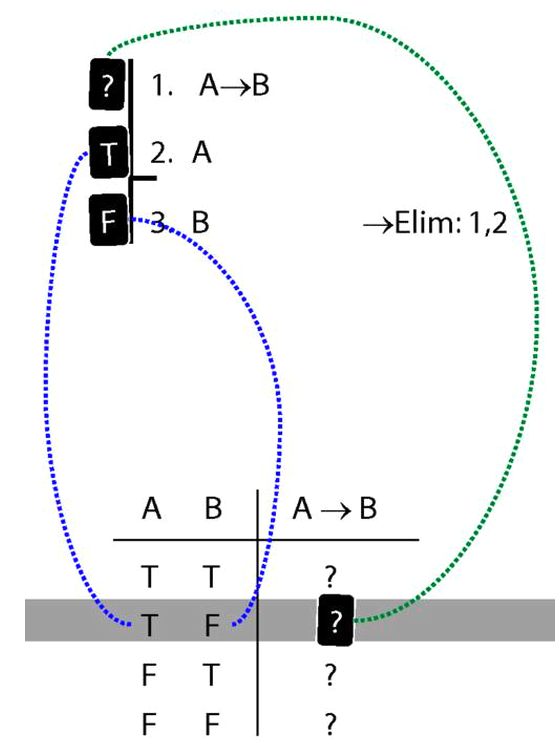
\includegraphics[scale=0.3]{img/unit_700_rule_to_tt.png}
\end{center}
 
 
\section{Not If}
 
\begin{center}
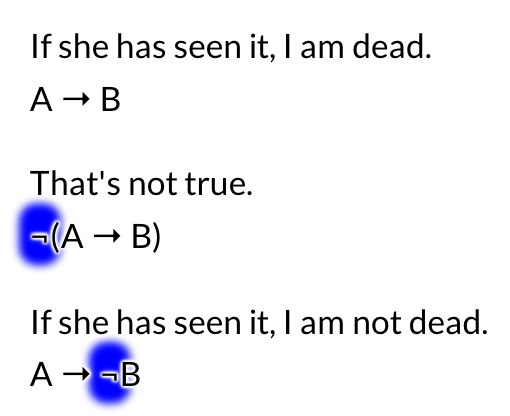
\includegraphics[scale=0.3]{img/not_if.png}
\end{center}
\begin{center}
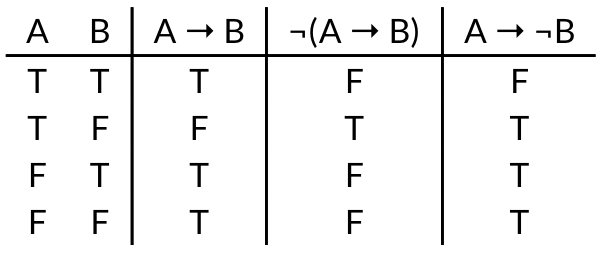
\includegraphics[scale=0.3]{img/not_if_tt.png}
\end{center}
 
 
\section{Fubar Rules}
 
\emph{Reading:} §8.3
 
\begin{minipage}{\columnwidth}
 
Consider this made-up rule:
 
\begin{center}
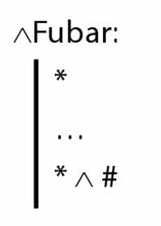
\includegraphics[scale=0.3]{img/fubar_rule.png}
\end{center}
Q1. What would be wrong with adding ∧Fubar to Fitch?
 
Q2. What would be wrong with having ∧Fubar in any system of proof?
 
\end{minipage}
 
 
 
\section{↔ : truth tables and rules}
 
\begin{center}
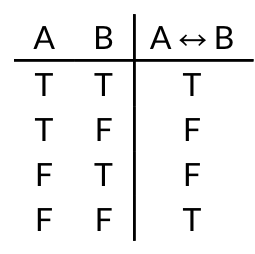
\includegraphics[scale=0.3]{img/tt_biconditional.png}
\end{center}
\begin{center}
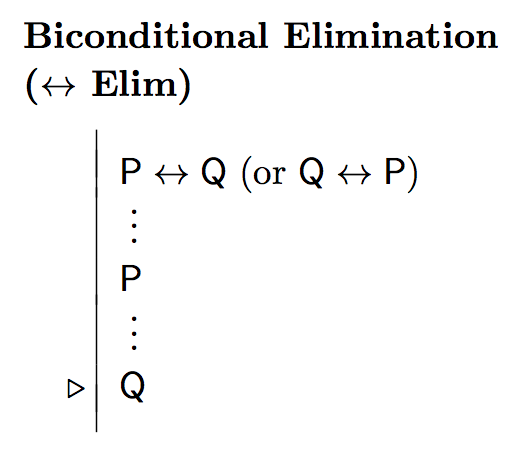
\includegraphics[scale=0.3]{img/rule_biconditional_elim.png}
\end{center}
\begin{center}
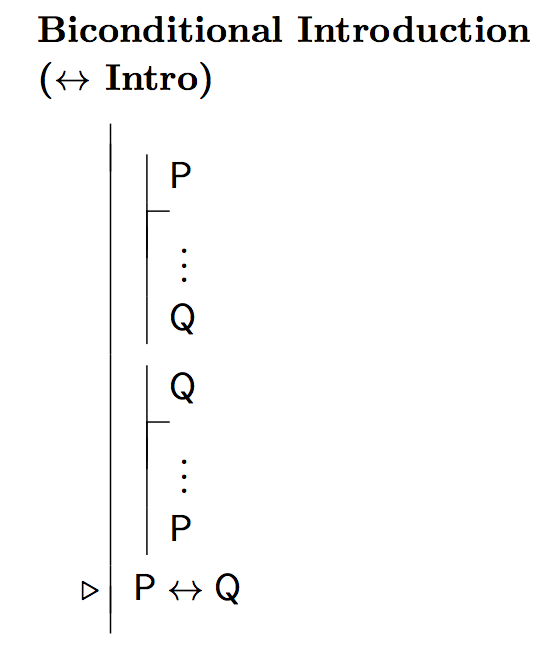
\includegraphics[scale=0.3]{img/rule_biconditional_intro.png}
\end{center}
 
 
\section{Translation with Quantifiers}
 
\emph{Reading:} §9.5, §9.6
 
\begin{minipage}{\columnwidth}
 
All discordians weep:
 
∀x( Dscrdn(x) → Wps(x) )
 
\end{minipage}
 
\begin{minipage}{\columnwidth}
 
All \textbf{quadrumanous} discordians weep:
 
∀x( ( \textbf{Quadr(x) ∧} Dscrdn(x) ) → Wps(x) )
 
\end{minipage}
 
\begin{minipage}{\columnwidth}
 
All quadrumanous discordians weep \textbf{and wail}:
 
∀x( ( Quadr(x) ∧ Dscrdn(x) ) → ( Wps(x) \textbf{ ∧ Wls(x)} ) )
 
\end{minipage}
 
\begin{minipage}{\columnwidth}
 
All quadrumanous discordians weep and wail \textbf{except Gillian Deleude}:
 
∀x( ( Quadr(x) ∧ Dscrdn(x) \textbf{∧ ¬(x=a)} ) → ( Wps(x) ∧ Wls(x) ) )
 
\end{minipage}
 
 
 
\section{∃Intro}
 
\emph{Reading:} §13.2
 
\begin{center}
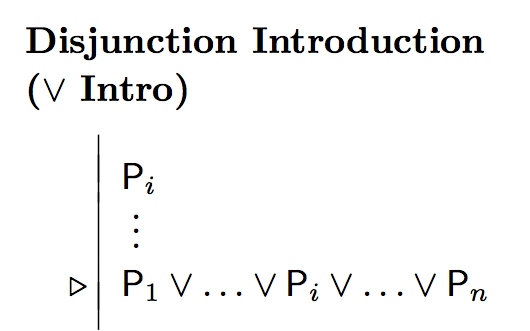
\includegraphics[scale=0.3]{img/rule_disjunction_intro.png}
\end{center}
\begin{center}
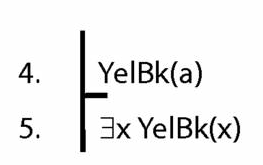
\includegraphics[scale=0.3]{img/unit_801_proof.png}
\end{center}
 
 
\section{What does ∃ mean?}
 
\emph{Reading:} §9.4
 
We give the meaning of ∃ by specifying what it takes for a sentence containing ∃ to be true:
 
\begin{enumerate}
 
\item Give every object a name.
 
\item For each name in turn, create a new sentence like this: delete the quantifier and replace all instances of the variable it binds with that name.
 
\item If ANY of the new sentences are true, so is the original sentence.
 
\end{enumerate}
 
 
 
\section{There Does Not Exist}
 
Something is not dead:
 
\hspace{3mm} ∃x ¬Dead(x)
 
Nothing is dead:
 
\hspace{3mm} ¬∃x Dead(x)
 
Everything is not broken:
 
\hspace{3mm} ∀x ¬Broken(x)
 
Not everything is broken:
 
\hspace{3mm} ¬∀x Broken(x)
 
\begin{center}
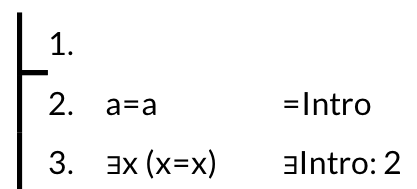
\includegraphics[scale=0.3]{img/unit_605_prf1.png}
\end{center}
\begin{center}
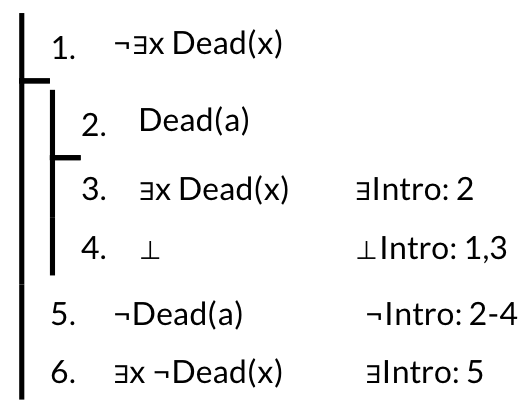
\includegraphics[scale=0.3]{img/unit_605_prf2.png}
\end{center}
 
 
\section{Quantifier Equivalences: ¬∀x Created(x) $\leftmodels\models$ ∃x ¬Created(x)}
 
\emph{Reading:} §10.1, §10.3, §10.4
 

%--- end paste
%--------------- 
 


\end{multicols*}

\end{document}